\documentclass[tikz]{standalone}
\usepackage{mrseqdia}


\begin{document}

% FID acquisition
\begin{tikzpicture}
  \init;
  \startline{1}{RF};
  \pulse{1}{1}{$\alpha$};
  \xline{0.5};
  \acq{3}{0.5}{Acquire};
  \xline{1};
\end{tikzpicture}

% Spin Echo Fragment
\begin{tikzpicture}
  \init;
  \startline{1}{RF};
  \pulse{1}{1}{$\alpha$};
  \xline{3};
  \pulse{1}{2}{$180^\circ$};
  \xline{2};
  \acq{3}{0.5}{Acquire};
  \xline{1};
  \xspan[(1.5,-2.1)]{4}{TE/2};
  \xspan{4}{TE/2};
  \yline[($(O) + (0,0.8)$)]{2.1};
  \echo[($(O) + (0,2.5)$)];
\end{tikzpicture}

% Gradient Echo Fragment
\begin{tikzpicture}
  \init;
  \startline{1}{RF};
  \pulse{1}{1}{$\alpha$};
  \xline{2};
  \acq{3}{0.5}{Acquire};
  \echo[($(O) + (-1.5,0.4)$)];
  \xline{1};

  \xspan[(1.5,-1.5)]{4}{TE};

  \startline[(0,-2.5)]{1.5}{Gx};
  \fgrad{2}{-0.5};
  \fgrado{2}{0.5};
  \yspan[($(O) + (0,-0.5)$)]{(5.5,-0.25)};
  \ograd{2}{0.5};
  \xline{0.5};
\end{tikzpicture}

% Slice-Selection Fragment
\begin{tikzpicture}
  \init;
  \startline{1}{RF};
  \pulse{1}{1}{$\alpha$};
  \xline{2.5};

  \startline[(0,-2)]{0.5}{Gz};
  \grado{1}{0.5};
  \ofgrad{1}{0.5};
  \fgrad{1}{-0.5};
  \xline{1};

  \yspan[(1.5,-2)]{(1.5,-1)};
  \xspan[(0.5,-3)]{2}{\scriptsize Ts};
  \xspan{1}{\scriptsize Ts/2};
\end{tikzpicture}

% Phase Encoding Fragment with Spin Echo
\begin{tikzpicture}
  % \draw[help lines] (-1,2) grid (12,-5);

  \init;
  \startline{1}{RF};
  \pulse{1}{1}{$\alpha$};
  \xline{3};
  \pulse{1}{2}{$180^\circ$};
  \xline{2};
  \acq{3}{0.5}{Acquire};
  \echo[($(O) + (-1.5,0.4)$)];
  \xline{0.5};

  \xspan[(1.5,-2.25)]{4}{TE/2};
  \xspan{4}{TE/2};
  \yspan{++(0,1.75)};

  \startline[(0,-3.5)]{2.75}{Gy};
  \phgrad{1.5}{0.5}{8};
  \xline{7.25};

  \xspan[(2.75,-4.5)]{1.5}{Tp};  
\end{tikzpicture}


% Phase Encoding Fragment with Spin Echo
\begin{tikzpicture}
  % \draw[help lines] (-1,2) grid (12,-5);

  \init;
  \startline{1}{RF};
  \pulse{1}{1}{$\alpha$};
  \xline{3};
  \pulse{1}{2}{$180^\circ$};
  \xline{2};
  \acq{3}{0.5}{Acquire};
  \echo[($(O) + (-1.5,0.4)$)];
  \xline{0.5};

  \xspan[(1.5,-2.25)]{4}{TE/2};
  \xspan{4}{TE/2};
  \yspan{++(0,1.75)};

  \startline[(0,-3.5)]{2.75}{Gy};
  \phgrad{1.5}{0.5}{8};
  \xline{7.25};

  \xspan[(2.75,-4.5)]{1.5}{Tp};  
\end{tikzpicture}


% Multislice SE volume acquisition
\begin{tikzpicture}
  % \draw[help lines] (-1,2) grid (15,-10);

  \init;
  \startline{1}{RF};
  \pulse{1}{1}{$\alpha$};
  \xline{3};
  \pulse{1}{2}{$180^\circ$};
  \xline{2.25};
  \acq{2.5}{0.5}{Acquire};
  \echo[($(O) + (-1.25,0.4)$)];
  \xline{0.75};

  \xspan[(1.5,-2.25)]{4}{TE/2};
  \xspan{4}{TE/2};
  \yspan{++(0,1.75)};

  \startline[(0,-3.5)]{2.75}{Gx};
  \fgrad{1.5}{0.5};
  \xline{3.75}
  \fgrado{1.5}{0.5};
  \ograd{1.5}{0.5};
  \xline{0.5}
  \xspan[(2.75,-4)]{1.5}{Tr/2};
  \xspan[(8,-4)]{3}{Tr};

  \startline[(0,-5.5)]{2.75}{Gy};
  \phgrad{1.5}{0.5}{8};
  \xline{7.25};
  \xspan[(2.75,-6.5)]{1.5}{Tp};

  \startline[(0,-7.5)]{0.5}{Gz};
  \grad{2}{0.5};
  \grad{1}{-0.5};
  \xline{8};
  \xspan[(0.5,-8.5)]{2}{Ts};
  \xspan{1}{Ts/2};
\end{tikzpicture}

% 3D GRE with EPI Factor 3
\begin{tikzpicture}[line width=1pt]
  % \draw[help lines] (-1,2) grid (12,-9);

  \init;
  \startline{1}{RF};
  \pulse{1}{1}{$\alpha$};
  \xline{1};
  \acq{2}{0.5}{Acquire};
  \echo[($(O) + (-1,0.4)$)];
  \xline{0.5};
  \acq{2}{0.5}{Acquire};
  \echo[($(O) + (-1,0.4)$)];
  \xline{0.5};
  \acq{2}{0.5}{Acquire};
  \echo[($(O) + (-1,0.4)$)];
  \xline{1};

  \xspan[(1.5,-1.5)]{2.5}{TE};
  \xspan{2.5}{TE};
  \xspan{2.5}{TE};

  \startline[(0,-3)]{1.5}{Gx};
  \grad{1.25}{-0.5};
  \grad{2.5}{0.5};
  \grad{2.5}{-0.5};
  \grad{2.5}{0.5};
  \xline{0.75};

  \startline[(0,-5)]{2}{Gy};
  \phgrad{0.75}{0.6}{4};
  \xline{2.375};
  \blib{0.25}{-0.25};
  \xline{2.25};
  \blib{0.25}{-0.25};
  \xline{3.125};

  \startline[(0,-7)]{2}{Gz};
  \phgrad{0.75}{-0.6}{8};
  \xline{8.25};
  \xspan[(2,-8)]{0.75}{Ts};
\end{tikzpicture}

% Echo Symbol
\begin{tikzpicture}[scale=1.2]
  \echo[(0,0)];
\end{tikzpicture}

\end{document}
